\section{Transformers}

% 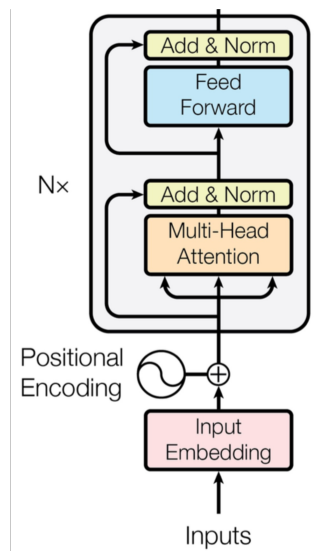
\includegraphics[width=0.3\linewidth]{images/transformer.png}

1. Attention:  
   \[
   \text{Attention}(Q, K, V) = \text{softmax}\left(\frac{QK^T}{\sqrt{d_k}}\right) V
   \] \\
2. Positional Embedding: High-freq sin / cos waves. \\

3. Vision Transformer (ViT): \\
   a. Patchify \& embedding: Images are divided into $16 \times 16$ patches. \\ 
   b. Learnable token [CLS] is prepended to every seq of patches. \\
   c. Classifier token is in the first $1 \times D$ row. \\
   d. Positional embeddings (PE) are learnable. \\
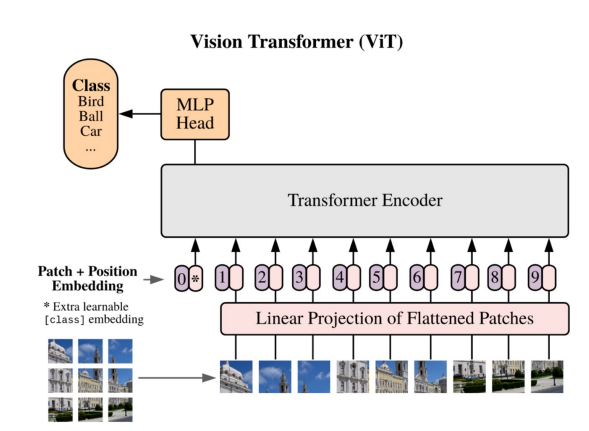
\includegraphics[width=1.0\linewidth]{images/vit.png}

4. Compact Transformers: \\
   a. \textbf{Sequence pooling:} \\
   1) Instead of adding [CLS] to seq, add it as an extra $D \times 1$ layer after encoder. \\
   2) Get Nx1 vec from NxD vec. \\
   3) Apply softmax to vec and mul w NxD vec $\to$ 1xD vec $\to$ classifier. \\
   b. Patchify + embedding $\approx$ conv with overlapping convolutions. \\

5. Examples: \\
   a. ViT-lite: Fewer layers/heads, smaller imgs. \\
   b. Compact Vision Transformer (CVT): Seq pool + conv layers. \\
   c. Convolutional Transformer (CCT): Less sensitive to PE due to convs. \\

6. Add Attention to Vision: \\
   a. Feed imgs to transformers. \\
   b. CNN + attention/self-attention layers. \\
   c. Replace CNN w/ attention or transformers (e.g., Swin Transformer). \\